\documentclass{report}

\input{~/dev/latex/template/preamble.tex}
\input{~/dev/latex/template/macros.tex}

\title{\Huge{}}
\author{\huge{Nathan Warner}}
\date{\huge{}}
\pagestyle{fancy}
\fancyhf{}
\lhead{Warner \thepage}
\rhead{}
% \lhead{\leftmark}
\cfoot{\thepage}
\setborder
% \usepackage[default]{sourcecodepro}
% \usepackage[T1]{fontenc}

\begin{document}
    % \maketitle
        \begin{titlepage}
       \begin{center}
           \vspace*{1cm}
    
           \textbf{Chapters 1-4}
    
           \vspace{0.5cm}
           Stat 128: Elementary Statistics
            
                
           \vspace{1.5cm}
   
           A Document By: \\
           \textbf{Nathan Warner}
    
           \vfill
                
                
           \vspace{0.8cm}
         
           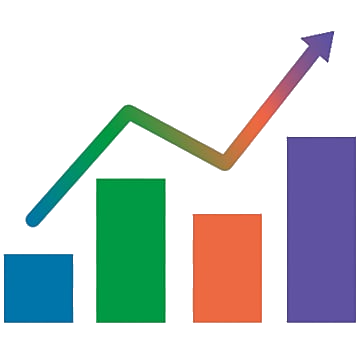
\includegraphics[width=0.4\textwidth]{./figures/2.png}
           \bigbreak \noindent 
            July 03, 2023  \\
           Computer Science \\
           Joliet Junior College \\
           United States\\
           
                
       \end{center}
    \end{titlepage}
    \tableofcontents
    \pagebreak \bigbreak \noindent
    \section{Learning Outcomes}
    \bigbreak \noindent 
    \textbf{Chapter 1:}
    \begin{enumerate}
        \item Define data collection techniques including observational studies and design of experiments.
        \item Identify appropriate sampling methods.
    \end{enumerate}
    \bigbreak \noindent 
    \textbf{Chapter 2:}
    \begin{enumerate}
        \item Differentiate qualitative and quantitative data graphically.  This includes graphs such as bar plots, histograms, and dot plots.
    \end{enumerate}
    \bigbreak \noindent 
    \textbf{Chapter 3:}
    \begin{enumerate}
        \item Calculate measures of central tendency for data.
        \item Explain the concept of resistance.
        \item Decide which measure of central tendency to report for various data sets.
        \item Determine measures of dispersion for data.
        \item Determine standard scores, percentiles, and quartiles.
        \item Identify outliers using quartiles.
        \item Interpret boxplots.
    \end{enumerate}
    \bigbreak \noindent 
    \textbf{Chapter 4:}
    \begin{enumerate}
        \item Evaluate the linear correlation coefficient for bivariate quantitative data.
        \item Evaluate whether the coefficient is significant at a given level.
        \item Explain the difference between correlation and causation.
        \item Determine the least-squares regression equation for a given set of bivariate data.
        \item Predict values of the dependent variable using the least-squares regression equation.
        \item Interpret the slope and intercept of the least-squares regression equation.
        \item Test the requirements of the least-squares regression model using residual analysis.
        \item Determine and interpret the coefficient of determination.
        \item Graphically analyze bivariate quantitative data for outliers and influential observations.
        \item Describe the association between two qualitative variables using conditional distributions.
        \item Explain Simpson’s Paradox.
    \end{enumerate}

    \pagebreak \bigbreak \noindent
    \section{Chapter 1:}

    \bigbreak \noindent 
    \subsection{1.1: Introduction to the Practice of Statistics}

    \bigbreak \noindent 
    \textbf{\textit{\underline{Objectives for this section.}}}
    \begin{enumerate}
        \item Define Statistics and Statistical Thinking
        \item Explain the Process of Statistics
        \item Distinguish between Qualitative and Quantitative Variables
        \item Distinguish Between Discrete and Continuous Variables.
    \end{enumerate}
    
    \bigbreak \noindent \bigbreak \noindent 
    \textbf{\textit{\underline{Define Statistics and Statistical Thinking:}}}
    \bigbreak \noindent
        Statistics is the science of collecting, organizing, summarizing, and analyzing information to draw conclusions or answer questions. In addition, statistics is about providing a measure of confidence in any conculsions.
        \bigbreak \noindent 
        \textbf{Note:} We must report a measure of our confidence in our results because we do not have 100\% certainty our answers are correct.
        \bigbreak \noindent 
        The information referred to in the definition above is \textit{data}. \textbf{Data} are a "fact or proposition used to draw a conclusion or make a decision." Data describes characteristics of an individual.
        \bigbreak \noindent 
        One crucial thing to understand about \textbf{data}, is that is \textbf{varies}. One thing that makes an interesting study is the fact that the data within the study varies. A study about number of hearts a human has is not only uninteresting but not worth doing. This is because the data does not vary.
        \bigbreak \noindent 
        \textbf{Two Major Goals:}
        \begin{enumerate}
            \item Describe Variablitiy.
            \item Understand sources of Variablitiy.
        \end{enumerate}
        \bigbreak \noindent 
        In Statistics, the same approach to solving a problem can still lead to different results. This does not happen in a math class.
        \vspace{1em}

        \bigbreak \noindent \bigbreak \noindent 
        \textbf{\textit{\underline{Explain the Process of Statistics.}}}
        \bigbreak \noindent 
        First lets define some vocabulary:
        \begin{itemize}
            \item \textbf{Population:} The entire group to be studied is called the population.
            \item \textbf{Sample:} In statistics, it is often impractical or impossible to get access to the entire \textbf{population}, which is why we only look at a \textbf{sample.} A sample is a \textbf{subset} of the population being studied.
            \item \textbf{Individual:} An individual is a person or object that is a member of the population being studied.
            \item \textbf{Statistic:} A statistic is a numerical summary of a sample.
            \item \textbf{Descriptive Statistics:} Descriptive statistics consist of organizing and summarizing data. Descriptive statistics describe data through numerical summaries, tables, and graphs.
            \item \textbf{Inferential Statistics:} inferential Statistics uses methods that take a result from a sample, extend it to the population, and measure the reliability of the result.
            \item \textbf{Parameter:} A parameter is a numerical summary of a population.
        \end{itemize}

        \bigbreak \noindent 
        \textbf{The process of statistics:}
        \begin{enumerate}
            \item Identify the problem to be solved. It is important to clearly lay out the questions that the researcher wants answered, along with cleary specifying which populution the study applies.
            \item Collect the data.
            \item Describe the data.
            \item Preform inference.
        \end{enumerate}

        \bigbreak \noindent 
        \begin{mdframed}
          \textbf{Example: The AP - National Constitution Center conducted a national poll to learn how adult Americans feel existing gun-control laws infringe on the second amendment to the U.S Constitution}
          \bigbreak \noindent 
          \textbf{The Following statistical process allowed the researchers to conduct their study.}
          \begin{enumerate}
              \item \textbf{Identify the research objective.}: The researchers wished to determine the percentage of adult Americans who believe gun-control laws infringe on the public's right to bear arms.
            \item \textbf{Collect the information needed to answer the question posed in (1).}: It is unreasonable to expect to survey the more than 200 million adult Americans to detrmine how they feel about gun-control laws. So the researchers surveyed a sample of 1007 adult Americans. Of those surveyed, 514 stated they believe existing gun-control laws infringe on the public's right to bear arms.
            \item \textbf{Describe the data.}: Of the 1007 induviduals in the survey, 51\% believe existing gun-control laws infring on the public's right to bear arms. This is a descriptive statistic, because its value is determined from a sample.
            \item \textbf{Preform inference.}: The reasearchers at the AP - National Constitution Center wanted to extend the results of the survey to \textbf{all} adult Americans. When generalizing results from a sample to a population, the results are \textbf{uncertain}. To account for this uncertainty, researchers reported a 3\% \textit{margin of error.} This means that the researchers feel fairly certain (in fact, 95\% certain) that the percentage of \textit{all} adult Americans who believe existing gun-control laws infringe on the public's right to bear arms is somewhere between 48\% and 54\%

          \end{enumerate}
          
        \end{mdframed}

        \bigbreak \noindent \bigbreak \noindent 
        \textbf{\textit{\underline{Distinguish between Qualitative and Quantitative Variables}}}
        \bigbreak \noindent 
        First let's define some vocab:
        \begin{itemize}
            \item \textbf{Variables:} The characteristics of the induviduals in a study. Variables vary, which means they can take on different values.
            \item \textbf{Constants:} Variables that do not vary. Inferential statistics is not necessary with constants.
        \end{itemize}
        \bigbreak \noindent 
        One goal of research is to learn the causes of variablitiy.
        \bigbreak \noindent 
        Variables can be classified into two groups: qualitative and quantitative.
        \begin{itemize}
            \item \textbf{Qualitative, or categorical variables} allow for the classification of individuals base on some attribute or characteristic.
            \item \textbf{Quantitative variables} provide numerical measures of induviduals. The values of a quantitative variable can be added or subtracted and provide meaningful results.
        \end{itemize}
        \bigbreak \noindent 
        \begin{mdframed}
          \textbf{Example: Determine whether the following variables are qualitative or quantitative.}
          \begin{enumerate}[label=\alph*.)]
              \item \textbf{Gender.}: Qualitative
              \item \textbf{Temeperature.}: Quantitative
              \item \textbf{Number of days during the past week that a college student studied.}: Quantitative
              \item \textbf{Zip Code.} Qualitative
          \end{enumerate}
          \textbf{Caution:} A numeric value does not automatically suggest a variable is quantitative.
        \end{mdframed}

        \bigbreak \noindent 
        \textbf{\textit{\underline{Distinguish between Discrete and Continuous Variables.}}}
        \begin{itemize}
            \item A \textbf{discrete variable} is a quantitative variable that has either a finite number of possible values or a countable number of possible values. A discrete variable cannot take on every possible value between any two possible values.
            \item A \textbf{continuous variable} is a quantitative variable that has an infinite number of possible values that are not countable. A continuous variable may take on every possible value between any two values. Continuous variables typically result from measurement. Continuous variables are often rounded. If a certain make of car gets 24 miles per gallon (mpg) of gasoline, its miles per gallon must be greater than or equal to 23.5 and less than 24.5, or $23.5 \leq mpg \leq 24.5$
        \end{itemize}

        \bigbreak \noindent 
        This Figure illustrates the relationship among qualitative, quantitative, discrete, and continuous variables.

        \begin{figure}[ht]
            \centering
            \incfig{graph1}
            \label{fig:graph1}
        \end{figure}

        \bigbreak \noindent 
        \begin{mdframed}
          \textbf{Example: Distinguish whether the quantitative variables are discrete or continuous.}
          \begin{enumerate}[label=\alph*.)]
            \item \textbf{The number of heads obtained after flipping a coin five times.}: Discrete
            \item \textbf{The number of cars that arrive at a McDonald's drive through between 12:00 PM and 1:00 PM}: Discrete
            \item \textbf{The Distance a 2011 Toyota Prius can travel in city driving conditions with a full tank of gas.}: Continuous
          \end{enumerate}
        \end{mdframed}

        \bigbreak \noindent 
        \textbf{Vocab:}
        \begin{itemize}
            \item The list of observed values for a variable is \textbf{data.}
            \item \textbf{Qualitative data} are observations corresponding to a \textbf{qualitative variable.}
            \item \textbf{Quantitative data} are observations corresponding to a quantitative variable.
            \item \textbf{Discrete data} are observations corresponding to a discrete variable.
            \item \textbf{Continuous data} are observations corresponding to a continuous variable.
        \end{itemize}

        \bigbreak \noindent 
        \begin{mdframed}
          \textbf{Example: Distinguish between Variables and Data}
          \bigbreak \noindent 
          The following table presents a group of seleted countries and information regarding these countries.
          \bigbreak \noindent 
          Identify the individuals, variables, and data.
          \begin{center}
              \begin{tabular}{|l|c|c|c|}
              \hline
              Country & Government Type & Life Expectancy (Years) & Population (in millions) \\
              	\hline
              Australia & Federal parliamentary democracy & 81.63 & 21.3   \\
              	\hline
            Canada & Constitutional monarchy & 81.23 & 33.5 \\
            \hline
            France & Republic & 80.98 & 64.4 \\
            \hline
            Morocco & Constitutional monarchy & 75.47 & 31.3 \\
            \hline
            Poland & Republic & 75.63 & 38.5 \\
            \hline
            Sri Lanka & Republic & 75.14 & 21.3\\
            \hline
            United States & Federal Republic & 78.11 & 307.2 \\
            \hline
              \end{tabular}
          \end{center}
          \bigbreak \noindent 
          \textbf{Qualitative}: Government Type \\
          \textbf{Quantitative}: Life Expectancy and Population \\
          \textbf{Continuous}: Life Expectancy \\
          \textbf{Discrete}: Population \\
          \textbf{Data}: Everything under Government Type, Life Expectancy, and Population.
      \item 
        \end{mdframed}

        \pagebreak \bigbreak \noindent
        \begin{center}
            \begin{large}
                \textbf{All Vocab / Concepts From Section 1.1}
            \end{large}
        \end{center}
        \line(1,0){490}
        \begin{itemize}
            \item \textbf{Population:} The entire group to be studied is called the population.
            \item \textbf{Sample:} In statistics, it is often impractical or impossible to get access to the entire \textbf{population}, which is why we only look at a \textbf{sample.} A sample is a \textbf{subset} of the population being studied.
            \item \textbf{Individual:} An individual is a person or object that is a member of the population being studied.
            \item \textbf{Statistic:} A statistic is a numerical summary of a sample.
            \item \textbf{Descriptive Statistics:} Descriptive statistics consist of organizing and summarizing data. Descriptive statistics describe data through numerical summaries, tables, and graphs.
            \item \textbf{Inferential Statistics:} inferential Statistics uses methods that take a result from a sample, extend it to the population, and measure the reliability of the result.
            \item \textbf{Parameter:} A parameter is a numerical summary of a population.
            \item \textbf{Variables:} The characteristics of the induviduals in a study. Variables vary, which means they can take on different values.
            \item \textbf{Constants:} Variables that do not vary. Inferential statistics is not necessary with constants.
            \item \textbf{Data:} The list of observed values for a variable.
            \item \textbf{Qualitative data} are observations corresponding to a \textbf{qualitative variable.}
            \item \textbf{Quantitative data} are observations corresponding to a quantitative variable.
            \item \textbf{Discrete data} are observations corresponding to a discrete variable.
            \item \textbf{Continuous data} are observations corresponding to a continuous variable.
        \end{itemize}

        \bigbreak \noindent 
        \textbf{Concepts:}
        \begin{itemize}
            \item Statistics and Statistical Thinking.
            \item Describe Variability
            \item Understand Sources of variablitiy
            \item Statistical studies are concerned with both describing the variability in the data and understanding the sources of variability in data. Understanding the sources allows researchers to control it and reach better conclusions.
            \item The process of statistics
            \item Inferential/Descriptive Statistics
            \item Variables
                \begin{itemize}
                    \item Qualitative (Categorical) / Quantitative
                    \item Discrete / Continuous
                \end{itemize}
            \item Data
                \begin{itemize}
                    \item Qualitative (Categorical) / Quantitative
                    \item Discrete / Continuous
                \end{itemize}
        \end{itemize}

        \pagebreak \bigbreak \noindent
        \subsection{1.2: Observational Studies versus Designed Experiments}
        \bigbreak \noindent 

    
\end{document}
